\documentclass[conference]{IEEEtran}
\IEEEoverridecommandlockouts
% The preceding line is only needed to identify funding in the first footnote. If that is unneeded, please comment it out.
\usepackage{cite}
\usepackage{amsmath,amssymb,amsfonts}
\usepackage{algorithmic}
\usepackage{graphicx}
\usepackage{textcomp}
\usepackage{xcolor}
\def\BibTeX{{\rm B\kern-.05em{\sc i\kern-.025em b}\kern-.08em
    T\kern-.1667em\lower.7ex\hbox{E}\kern-.125emX}}
\begin{document}

\title{Fast dynamic predecessor query on GPU}

\author{\IEEEauthorblockN{1\textsuperscript{st} Hubaut Youri}
\IEEEauthorblockA{\textit{Computer Science} \\
\textit{Université Libre de Bruxelles}\\
Brussels, Belgium \\
youri.hubaut@ulb.ac.be}
\and
\IEEEauthorblockN{2\textsuperscript{nd} Iacono John}
\IEEEauthorblockA{\textit{Computer Science} \\
\textit{Université Libre de Bruxelles}\\
Brussels, Belgium \\
johniacono@gmail.com}
}

\maketitle

\begin{abstract}
We present two dynamic dictionary data structures for the GPU, one offering \textit{constant time} operations based on X-fast tries and one other in constant-like time with a classical Hash Array Mapped Trie (HAMT). They present different characteristics, with their own advantages and inconvenients, and achieve performance at least equivalent to that of GPU Log Structured Merge tree (LSM), a previously introduced data structure, for look-up queries. They intend to be the first dictionaries to offer the element-wise updates and to exploit the notions of warp-parallelism.
\end{abstract}

\begin{IEEEkeywords}
Dictionary, GPU, dynamic, X-fast trie, HAMT, concurrent, LSM
\end{IEEEkeywords}

\section{Introduction}
Static data structure construction is common in GPU programming~\cite{alcantara2009real} because of the many problems that can arise when updating those in a highly concurrent environment, completely rebuild the structure at each update greatly simplifies the task while offering sufficiently correct performance. It is also classical to perform updates on the CPU side before sending it back to the GPU~\cite{li2013gamt}.

We therefore try to provide a data structure purely on the GPU side and capable of supporting modifications in a highly concurrent context, while ensuring its correctness and remaining competitive to a complete reconstruction. Specifically, the dictionary is a category of abstract data type which is relatively basic but can solve many problems and can be used for other purposes as a priority queue; a GPU oriented version would increase the number of problems that could be handled by them and thus improve their field of application.

In this paper, we will begin by introducing the first proposed dictionary, offering operations in constant time with its main ideas. We will then present a second, much more classical and simple, data structure but which nevertheless offers very good performances in practice. Finally, we will compare performance against two other data structures.

\section{Background and previous work}

GPUs have now been used for some years as General-purpose processing on graphics processing units (GPGPUs). Indeed, they present massive and lightweight parallelism at low cost, with an excellent power consumption ratio and latency hiding. Thousands of threads can easily be executed simultaneously while abstracting the hardware from the running program.

This parallelism is found at several levels but the smallest unit corresponds to the ``warp'' which is executed in lockstep. That is, the same instruction is executed on several threads at once, which means that if there are divergences in the computations, each branch will be executed sequentially, the result not being kept for threads that have not taken the branch.

These warps present a mechanism of elections allowing all threads in a warp to perform a broadcast operation followed by a reduction in a single step and at very high speed. Each thread can, for example, compare the value of an integer with a reference value, the results are then combined and sent to each participant. It is then enough to recover the position of the bits set to one to know for which threads the predicate was true.

\section{GPU X-fast trie}

In this paper, we propose a GPU dictionary data structure whose operations are in constant time. This one is based on the X-fast tries introduced by D. E. Willard~\cite{willard1983log} as variants for the van Emde Boas trees~\cite{van1975preserving}. The idea being to exploit warp-parallelism in order to find the information related to each level at the same time.

\subsection{X-fast trie}

The X-fast tries were introduced by D. E. Willard to improve the memory consumption of the van Emde Boas trees and to serve as the base component for his Y-fast tries. This is a type of data structure that supports dictionary operations for integers belonging to a bounded domain of size $u$, a universe. The X-fast tries principle is relatively simple, we save all the prefixes of each element introduced in different hash tables according to their length.

\iffalse 
\begin{figure}[htbp]
\centerline{\includegraphics[width=0.5\textwidth]{xfasttrie-warp.png}}
\caption{X-fast trie structure with elements 2, 3 and 6.}
\label{fig}
\end{figure}
\fi

There are two types of levels in the tree, internal nodes and leaves. The leaves are used to store the elements and are conceptually attached together through a doubly linked and sorted list. Internal nodes only appear if their prefix lead to a terminal leaf and are used for predecessor or successor queries, they allow to be directed to the minimum or maximum element of the subtree.

This structure naturally introduces complexity in $O(\log u)$ for insertions and deletions, $O(\log \log u)$ for predecessors or successors queries thanks to a binary search on the prefixes and $O(1)$ for searches and this for memory consumption in $O(N \log u)$. Y-fast tries are theoretically better thanks to their $O(\log \log u)$ for updates and their consumption in $O(N)$  but they didn't have an essential feature.

Indeed, we wanted to exploit warp-parallelism effectively and we therefore wanted every thread belonging to the same warp to be able to participate in the current operation. The idea emerged to use each thread simultaneously in order to find the information related to the prefixes. The advantage is that all threads will perform the same tasks but on different hash tables, which will decrease the divergence.

It only remains to determine which threads have found their relative prefix or not through the election system and update the trie accordingly, updating the top nodes of the trie and adding those missing until the newly added leaf. Complexity becomes $O(\frac{\log u}{w})$, where $w$ is the size of a warp. Leaf operations are more sequential but can also benefit from warp-parallelism with the different probes of open addressing hash table for instance.

\subsection{Concurrency}

We looked if there was any work on concurrency for X-fast tries, it would seem there was only one prior work, with the so-called \textit{skip-trie} by R. Oshman and N. Shavit~\cite{oshman2013skiptrie}, due to their inherent difficulty and lack of practical application. Formal proof seems very difficult for this data structure.

Many problems can occur with these trees in a concurrent setting. Especially since we read several levels at once and the states can therefore be inconsistent if deletions are interleaved with other operations. It seems difficult to ensure consistent reading in many concurrent hash tables. A framework where the elements are not removed but simply invalidated would seem easier to put into practice, but will imply regular cleaning.

However, besides deletions, operations on internal nodes should not cause too many problems. We will always be able to determine where the prefixes begin to diverge. The principal difficulties will occur at the leaf level, where keeping the doubly linked and sorted list will present a real challenge. Indeed, the information on the predecessor and successor that is used for both insertion and search of these may no longer be optimal. We would find ourselves with a greater interval than expected and not the direct predecessor and successor. It may be interesting to restart the procedure from the beginning if the list traversal to arrive at a correct position does not end in a certain number of steps. Note that it is important to insert the element as soon as you update the information of an internal node to avoid searching for not yet fully inserted nodes and update its actual predecessors and successors immediately after.

\section{Hash Array Mapped Trie}

The second data structure that we introduce is much more classic and simple and is close to the idea behind Hash Array Mapped Trie~\cite{bagwell2001ideal}. The idea is close to a radix tree, we consider the first $k$ bits of the integer we want to add, if the position is empty, we create a new node, otherwise, we follow the pointer and we continue with the following bits. The essential difference is that the tree depth is fixed and that it is a bitmap, only the presence of the element is recorded. The data is stored in an external hash table.

The whole is optimized for the GPU, the data is grouped together and has for size a multiple of that of the cache lines; the internal nodes contain at least $w$ pointers and the leaves $w$ bits, where $w$ is the size of a warp. This information is essentially used for predecessor queries where we use the warp election mechanism to determine if there is a predecessor in the node and which one it is to continue our search if it fails. Similarly for leaves, if no predecessor is found, we just need to find the maximum element from the last predecessor pointer observed.

Concurrency is very simple to manage. The guarantees on insertions, deletions and searches are the same as in a traditional hash table. Predecessor queries can be redone entirely if they fail and this as long as there is a predecessor, but this event should be exceptional. We expect that a formal proof can be easily feasible in practice.

\section{Implementation details}

In this section, we will discuss in more detail the implementation of these data structures by reviewing each of the operations. Our design decisions have been influenced by the technical characteristics of GPUs and the development environment (CUDA). All operations are performed on chip in order to offer something more easily exploitable and can be performed with warp granularity.

\subsection{X-fast tries}

Implementing X-fast tries is complex, and make it correct seems even more difficult. We have tried to do our best but we do not guarantee that it is flawless, especially for insertions. We also dealt with the problem in a bulk case, where only insertions are made before queries and the operations are not mixed, even if we expect real problems when deleting.

\subsubsection{Hash table}

We developed and compared different models of concurrent hash tables to see which offered the best performance for our problem. We needed to be able to perform operations based on a single thread and to have an \textit{upsert} (insert or update) operation. It is all the more important to have efficient hash tables because the time of all warp searches will be determined by the slowest thread. We opted for classic models: open addressing, cuckoo hashing and chaining and we observed that open addressing with linear probing offered the best compromise following a relatively low load factor (50\%) and thanks to a certain stability of iterators.

\subsubsection{Insertion}

The insertions are divided into three stages. We start by looking for the level from which the existing prefixes start to diverge from the new element, it is enough to test the presence in each level simultaneously. Once the level is found, all the missing intermediate nodes are added up to the leaf. Then, we update the information of the top nodes, we chosed to save each time the minimum and the maximum of the subtree in the nodes. Finally, we insert the element at the leaf level and we try to add it to our doubly linked list. We have obtained an interval of nodes thanks to the largest prefix found, and we are trying to insert it in this space. We have to be careful and insert yourself as a neighbor with the instruction \textit{compare and swap}.
It is possible that many nodes are inserted in the same subtree and the path to find the right position in this list can be long. It can then be interesting to redetermine the smallest interval by doing a new predecessor query. In addition, a certain fairness must be established in the warp scheduling to avoid that we get the information from an updated node but the element is not yet inserted in the leaves.

\subsubsection{Deletion}

Deletion is less clear. Either one opts for an invalidation of the data at the level of the leaves, in this case, the work is immediate. Either, we need to delete all the nodes that have no children other than the one you want to remove and then update the information of the top nodes accordingly, this can be long. The last step consists to actually delete the item at the leaf level and update the list.

\subsubsection{Queries}

Searches are trivial and are limited to one query in a hash table. Predecessor queries are not so much more complicated; in particular, we recorded the minimum and maximum of each subtree in each of the nodes. Once you have found the level where the prefixes differ, you still have to potentially access the previous element if you are looking for the predecessor and there are no left child, for example. Count queries can be implemented by adding a counter in each of the nodes. Range queries are implemented in a lazy way, it is not possible to recover even part of a range at once. You need to iterate on each of the elements using the doubly linked list.

\subsubsection{Design}

We considered two different strategies for implementation. One where each level was stored separately. And the other where we group the information of neighboring levels together. In particular, the \textit{group size} is defined as the number of levels grouped into one, the first strategy being a special case where the number of merged levels is zero. The different levels are stored in a van emde boas layout~\cite{brodal2002cache} way. The idea was to minimize the number of cache lines we have to load to get our information.

\subsection{Hash Array Mapped Trie}

Hash Array Mapped Trie are much simpler. They are composed of two elements, internal nodes and leaves. The leaves contain the associated bits indicating the presence or not of the elements in the hash table and the intermediate nodes allow access to the appropriate leaf if it exists. All that remains is to dynamically allocate the tree elements according to needs.

When inserting and at the internal nodes, if two threads try to access a missing child in an internal node, one will allocate this new node while the other will wait for the new value. This can obviously introduce some contention, but we can argue that the probabilities are relatively low and we observe that the effects remain marginal.

We also opted for leaves to contain a multiple of 1024 bits at a time (10 bits of the integer) as a minimum since this corresponds to the size of a line cache. Each thread of the warp takes care of its 32-bit subinterval, the relative position being determined by its thread id. For intermediate nodes, we considered 64 pointers (corresponding to 6 bits) per node, which sets the depth of our tree to 5 levels for 32-bit keys.

\section{Performance evaluation}

\subsection{Other structures for comparison}

We wanted to compare the two data structures we had developed with two other data structures that offered similar operations (dictionaries) and sufficiently similar characteristics (exploiting the possibilities offered by graphic cards, in particular). We opted on the one hand for the B+-trees~\cite{fix2011accelerating} for their well-known properties~\cite{bender2005cache}, and on the other hand, for the recently introduced GPU LSM~\cite{ashkiani2017gpu}.

We started by implementing a B+-tree in a non-concurrent and thus sequential framework. We haven't considered a concurrent version despite some fairly effective models exist~\cite{braginsky2012lock}, so the inserts won't be directly comparable. However, we will exploit the parallelism offered by graphics cards for queries. We used a tree where there are 32 children per node.

We also developed a LSM GPU ourselves following author's indications. Implementation and performance may therefore differ from theirs. However, we used smaller batch sizes than those described in their article since we were limited by the size of the shared memory (for the sorting operation). We could launch only up to 512 threads at a time for insertions. We also did not want to test a more concurrent version where several blocks could contribute to this task given the contention that it seems to exist.

In the following sections, we will discuss performance for insertions, then searches and finish on predecessor queries. All experiments are performed on an NVIDIA GTX 1050ti, Pascal architecture with 4GB of DRAM (ECC disabled), and an AMD ryzen 5 1600 for processor. All programs have been compiled with NVIDIA's nvcc compiler (version 9.1.85) with the default optimization flags (for release) on Windows 10.

All the memory is pre-allocated, the hash tables are pre-constructed to contain all the data with a load factor of 50\%, same for the LSM buffers. A basic memory allocation mechanism is also used, a simple linear allocator where we allocate the following space each time (no deallocations).

\subsection{Insertions}

For the insertions, we have set up a simple experimental protocol. We want to insert a certain number of elements (with 32-bit keys) and we look at the time taken to complete this task. X-fast trie and HAMT are launched with a configuration of 16 warps (due to a limit on the number of registers available) and 32 blocks. LSM GPUs use batches of size 512 ($2^{9}$), so only 16 warps are executed in a single block. We collected data on 30 experiments. We were only able to test up to $2^{19}$ elements due to the excessive memory consumption of the X-fast tries which reached the limits of our system.

\begin{figure}[htbp]
\centerline{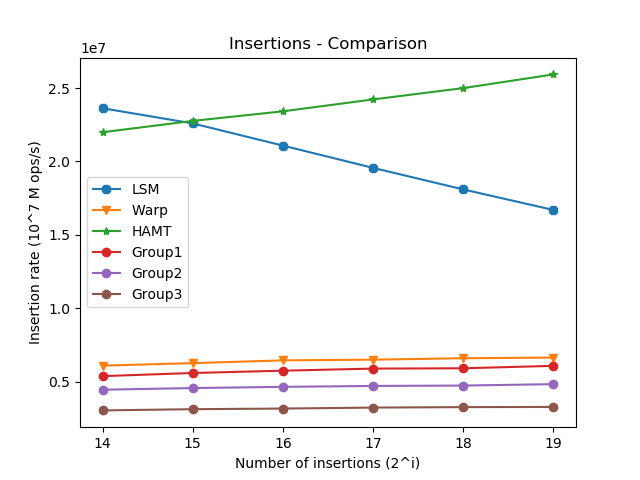
\includegraphics[width=0.5\textwidth]{InsertionRate1.png}}
\caption{Insertion rate versus total number of inserted elements.}
\label{InsertionRate}
\end{figure}

We can observe several phenomena on this graph. X-fast tries offer a more or less constant time to insert the elements. The efficiency of the LSM is reduced with the increasing number of elements due to the merging cascade and, on the contrary, the HAMT improve since it is less and less necessary to allocate a new node in the tree.

The X-fast tries still seem to offer a sufficiently interesting insertion rate (5M elements/s). The strategy of grouping different levels together do not seem to add any benefit (Warp vs GroupK). This is related to the fact that most of the time is lost in data depedencies of hash tables and that grouping elements does not help atomic operations used to ensure the correctness of the structure. We observe that the HAMT present the best performances (25M elements/s) but we insist on the fact that we are in a very unfavourable case with the LSM (small batch size - 20M elements/s) and that, in other circumstances, we expect those to be faster.

\subsection{Searches}

For searches, we first build the tested data structure with random data. We then collect the time taken to perform the searches with a total of 5 iterations, over 20 runs (which determine the distribution of the data) and with a configuration of 16 warps and 32 blocks. We considered the LSM in two cases, first in the most favorable setting where a power of 2 number of batches was inserted ($b2^{k}$ elements) and the most unfavorable where each level contains data (which correspond to $b(2^{k} - 1)$ elements). For X-fast tries and HAMT, both use the same hash table and therefore have the same performance.

\begin{figure}[htbp]
\centerline{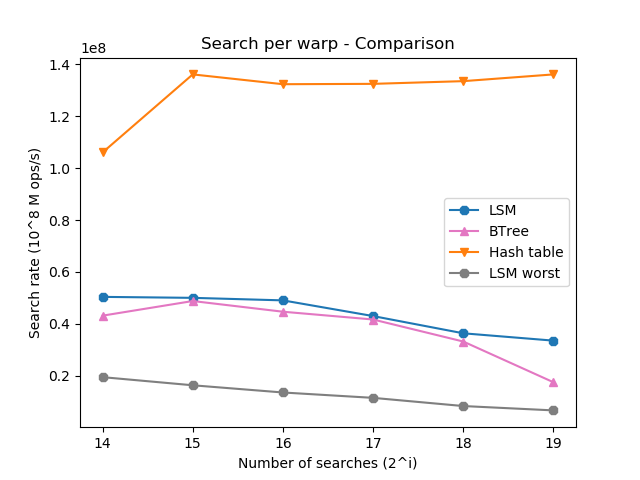
\includegraphics[width=0.5\textwidth]{SearchRate1.png}}
\caption{Search rate versus total number of searched elements.}
\label{Search rate}
\end{figure}

The results are quite natural, the hash table logically provides the best performance (140M elements/s). The B+-trees remain comparable in time to the most favorable case of the LSM before losing in performance (40M elements/s), this is related to the addition of a new level in the tree. Otherwise, relatively similar performance is not a surprise. Finally, the worst case of LSM results in a real performance loss that increases greatly with the number of elements (only 7M elements/s).

\subsection{Predecessor queries}

Finally, we look at the performance of the predecessor queries. Similarly, we can have a better and a worse case for LSM. We used the same experimental conditions than for searches, the value used for our predecessor request is randomly determined as a combination between the seed of the run and the current request number (we observed less than 0.01\% exact match).

\begin{figure}[htbp]
\centerline{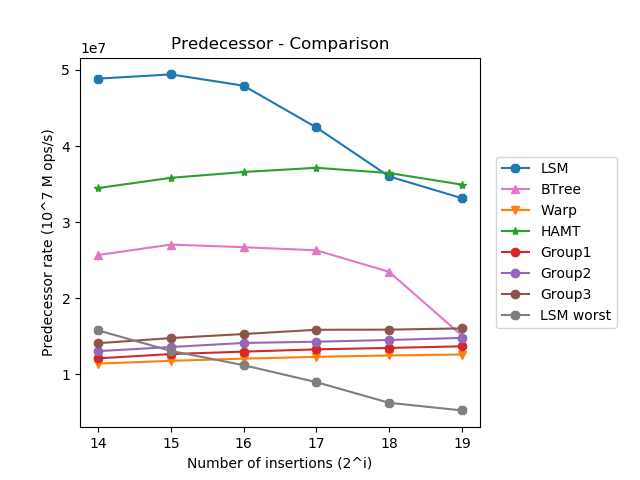
\includegraphics[width=0.5\textwidth]{PredecessorRate1.png}}
\caption{Predecessor rate versus total number of queried elements.}
\label{Predecessor rate}
\end{figure}

We observe the constant aspect for HAMT (35M elements/s) and X-fast tries (15M elements/s). For B+-trees (25M elements/s) and LSM (35M elements/s for best case and 5M elements/s for worst), we observe the same phenomenon as for searches, which is quite logical following strongly similar operations. Predecessor queries are slightly more complex than searches but they both use a lower bound algorithm and therefore performance is roughly the same. Contrary to the insertions, we notice that grouping the elements in the X-fast tries allows to gain some performances since we load a little less cache lines.

\section{Conclusion}

We have introduced and developed two new data structures that can be used as a GPU dictionary, allowing insertion of one element at a time while providing correct performance. They are proving to be real competitors to LSM while providing more flexibility, even though we still expect the LSM to be much faster for insertions. We note, however, that they have very different characteristics.

\subsection{X-fast tries}

X-fast tries have relatively low performances, despite constant time operations, they remain below what is proposed by LSM (on average) or HAMT. The big black point is that this data structure consumes a huge amount of memory and there doesn't seem to be enough room to deal with a real problem. Many atomic operations are also required in order to ensure its correctness and proving implementation seems like a very difficult task.

On the other hand, there is still room for possible improvements. If someone finds a better hash table, performance will be directly impacted, unlike more complex like B+-trees, it scales quite good. One can also hope that asymptotically, this structure presents a real interest with the key size increase. It is also easier to make the range queries than for HAMT.

\subsection{Hash Array Mapped Tries}

HAMT have shown excellent performance in all cases. They have the advantage of consuming relatively little memory and having constant time operations. Proving their correctness also seems much simpler. However, it is expected that if the size of the keys increases, they will suffer much more in terms of performance than the other data structures presented here. Range queries seem difficult to carry out in this context too. Much work has been done for the latter to provide a more dynamic and non-fixed structure. High-performance implementations with proof of correctness have also been proposed~\cite{prokopec2017cache}.

\bibliographystyle{IEEEtran}
\bibliography{bibliography.bib}

\end{document}
